%=======================================================
\section{Automatisches Service-Recovery}
%=======================================================
Der Einsatz von OpenNMS wird hauptsächlich zu reinen Überwachungszwecken von IT-Systemen verwendet. In manchen Umgebungen kann es hilfreich sein, wenn einfache Wiederherstellungsmassnahemn automatisch ausgeführt werden. Erst wenn diese zu keinem Erfolg führen, wird Benachrichtigung an einen Bereitschaftsmitarbeiter ausgelöst. In diesem Beispiel wird beschrieben wie eine OpenNMS Eskalations-Hierarchie verwendet werden kann um einen solchen Anwendungsfall abzubilden.

WARNUNG: Bei der Umsetzung sollte klar sein, was es bedeutet automatisch ins System einzugreifen und Systemkommandos über entfernte Rechner auszuführen. Zusätzlich sollten Seiteneffekte bezüglich Sicherheit und kennwortloser SSH-authentifizierung berücksichtigt werden. Die Funktionsweise der Eskalation und Benachrichtigung in OpenNMS sollte bekannt sein. Bitte anwenden, wenn Sie wissen was Sie tun.


%=======================================================
\subsection{Beispielszenario mit Web-Servern}
%=======================================================
Im folgenden wird das Konfigurationsszenario kurz beschrieben. In dem gezeigten Beispiel gibt es eine Reihe wichtiger und weniger wichtiger Webserver auf denen Apache2 ausgeführt wird. Die wichtigen Server sind in einer \emph{Surveillance Category} mit der Bezeichnung \emph{VIP-HTTP} zusammenfasst. Für einen Ausfall des Dienstes \emph{HTTP} versucht \emph{OpenNMS} drei mal den \emph{apache2} Dienst neu zu starten bevor eine \emph{SMS\abbrev{SMS}{\markup{S}hort \markup{M}essage \markup{S}ervice}} an den Administrator versendet wird. die folgende Abbildung stellt das Szenario kurz dar.

\begin{figure}[H]
	\centering
	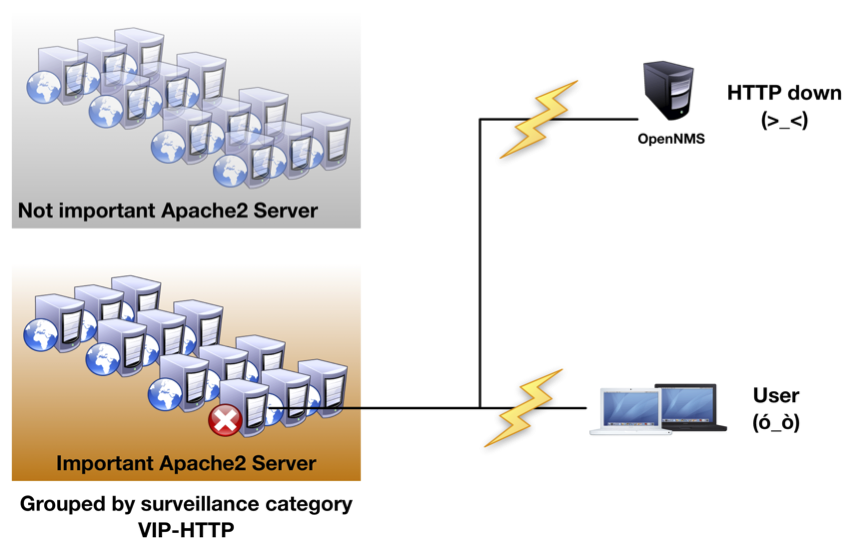
\includegraphics[width=1.0\textwidth]{images/use-cases/service-recovery/szenario}
	\caption{Wiederherstellung am Beispiel von Apache Web-Servern}
	\label{pic:szenario-recovery-apache}
\end{figure}

Für die Einrichtung sind die im folgenden beschriebenen Voraussetzung notwendig. Der Ablauf stellt sich wie folgt dar:

\begin{figure}[H]
	\centering
	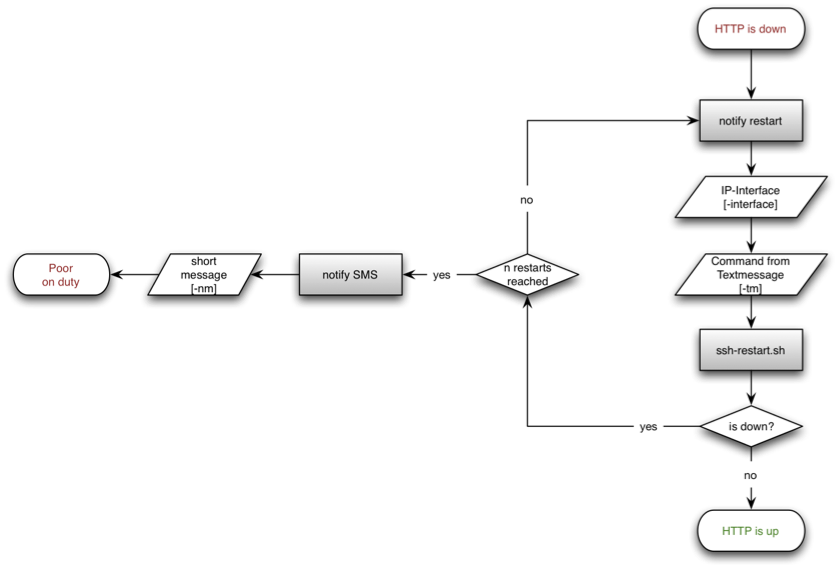
\includegraphics[width=1.0\textwidth]{images/use-cases/service-recovery/notification-workflow}
	\caption{Ablaufdiagram der Benachrichtigung mit Eskalation zur Wiederherstellung des Apache Web-Servers in OpenNMS}
	\label{pic:workflow-recovery-apache}
\end{figure}

%=======================================================
\subsection{Voraussetzungen}
%=======================================================
Der \emph{OpenNMS} Server muss in der Lage sein, entfernte Kommandos per \emph{SSH} ohne Kennworteingabe ausführen können. Dazu kann eine \emph{pubkey-Authentifizierung} eingerichtet werden. Wie \emph{pubkey-Authentifizierung} mit \emph{ssh-keygen} unter Linuxdistributionen eingesetzt wird hier nicht weiter behandelt und auf die Internetseite \url{https://help.ubuntu.com/community/SSH/OpenSSH/Keys} verwiesen. Es ist wichtig, dass \textbf{\textit{KEINE}} \emph{passphrase} verwendet werden darf.

Um einen Serverdienst unter \emph{Linux} neu starten zu können wird übelicherweise eine init-Skript verwendet. In unserem Beispiel wird \emph{Apache2} verwendet. Das init-Skript welches beim Systemstart verwendet wird liegt in 

\begin{lstlisting}[numbers=none]
/etc/init.d/apache2 start|stop|restart
\end{lstlisting}

Der Parameter \emph{restart} kann genutzt werden um einen bereits gestoppten oder fehlerhaft laufenden \emph{apache2} Prozess neu zu starten. Ein \emph{Wrapper-Script} übernimmt diese Aufgabe und kann wie folgt aussehen:

\lstinputlisting[caption={\emph{Wrapper-Skript} um einen service per \emph{SSH} entfernt neu starten zu können}
      \label{lst:ssh-restart-skript}]
  {configs/use-cases/service-recovery/ssh-restart.sh}

Das Skript erwartet drei Parameter und kann wie folgt ausgeführt werden:

\begin{lstlisting}[numbers=none]
ssh-restart.sh <ip-interface> <init-skript> <restart-command>
\end{lstlisting}

Wenn das Kommando vom \emph{OpenNMS} Server auf den zu überwachenden Webserver funktioniert kann mit der Konfiguration der Benachrichtigung in OpenNMS fortgefahren werden.

%=======================================================
\subsection{Benachrichtigung erweitern}
%=======================================================
Das oben gezeigt Skript kann jetzt als neues Kommando für die Benachrichtigung eingerichtet werden. Dazu wird die Datei

\begin{lstlisting}[numbers=none]
$OPENNMS_HOME/etc/notificationCommands.xml
\end{lstlisting}

bearbeitet. \textbf{\textit{Wichtig!}} Es ist darauf zu achten, dass die Pfadangabe in \emph{<execute>...</execute>} korrekt ist.

\lstinputlisting[caption={Benachrichtigung in OpenNMS mit \emph{ssh-restart.sh} erweitern}
      \label{lst:config-notificationCommands}]
  {configs/use-cases/service-recovery/notificationCommands.xml}

Über die \emph{-interface} und \emph{-tm} können über die Benachrichtigung die beiden wichtigen Parameter für unser \emph{SSH-Skript} mit übergeben werden. Nach einem Neustart kann unser \emph{restart-service} im \emph{Destination Path} ausgewählt werden.

%=======================================================
\subsection{Eskalation einrichten}
%=======================================================
Wir erzeugen in der Weboberfläche einen neuen \emph{Destination Path} mit der Bezeichnung \emph{restart-service}. Über die Eskalation wird festgelegt, wie oft versucht werden soll den Dienst neu zu starten. In der folgenden Abbildung ist die Konfiguration dargestellt. Über einen Benutzer \emph{remote} wurde kenntlich gemacht, dass hier ein remote-Kommando drei mal in einem 5-minütigem Abstand ausgeführt werden soll. Falls der \emph{HTTP-Dienst} nach dem dritten mal noch nicht wiederhergestellt ist, wird eine \emph{SMS} an den Benutzer \emph{indigo} gesendet.

\begin{figure}[H]
	\centering
	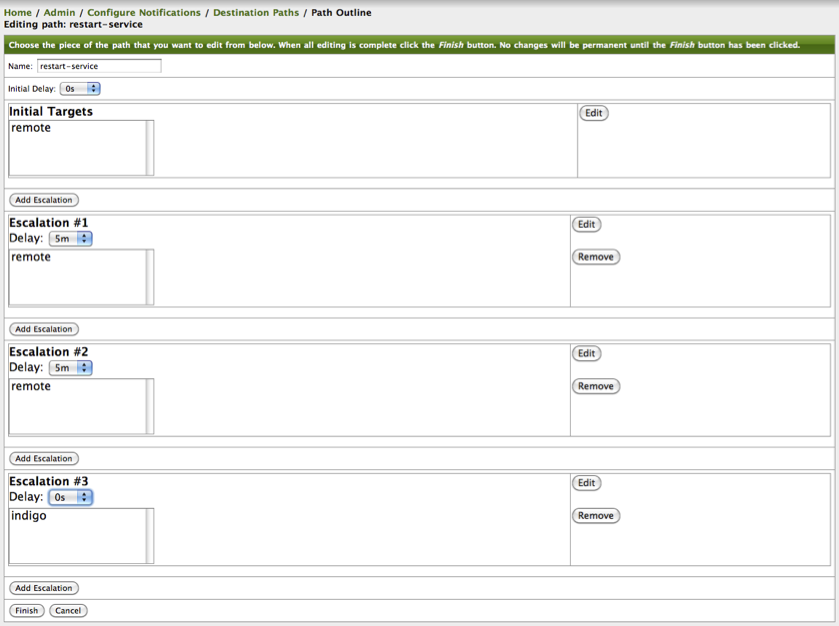
\includegraphics[width=1.0\textwidth]{images/use-cases/service-recovery/escalation}
	\caption{Eskalation für \emph{service-restart} Benachrichtigung}
	\label{pic:escalation-service-restart}
\end{figure}

\textbf{\textit{Wichtig!}} Für den Benutzer \emph{remote} ist zu beachten, dass kein Kommando ausgeführt wird, wenn der Dienst wieder verfügbar ist. Daher hier den Schalter auf \emph{off} setzen. Damit wird verhindert, dass Benachrichtigungen für \emph{RESOLVED-Events} gesendet werden.

\begin{figure}[H]
	\centering
	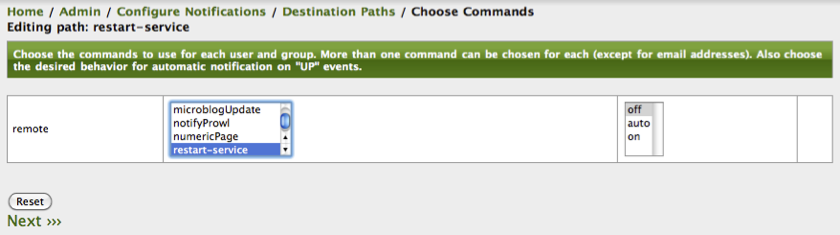
\includegraphics[width=1.0\textwidth]{images/use-cases/service-recovery/destination-path}
	\caption{Konfiguration eines \emph{Destination Path} für \emph{Service-Recovery}}
	\label{pic:destination-path-service-restart}
\end{figure}

Die Benachrichtigung für \emph{SMS} kann wie gewohnt eingerichtet werden. Im nächsten Schritt wird die Konfiguration für das \emph{nodeLostService Event} beschrieben.

\begin{figure}[H]
	\centering
	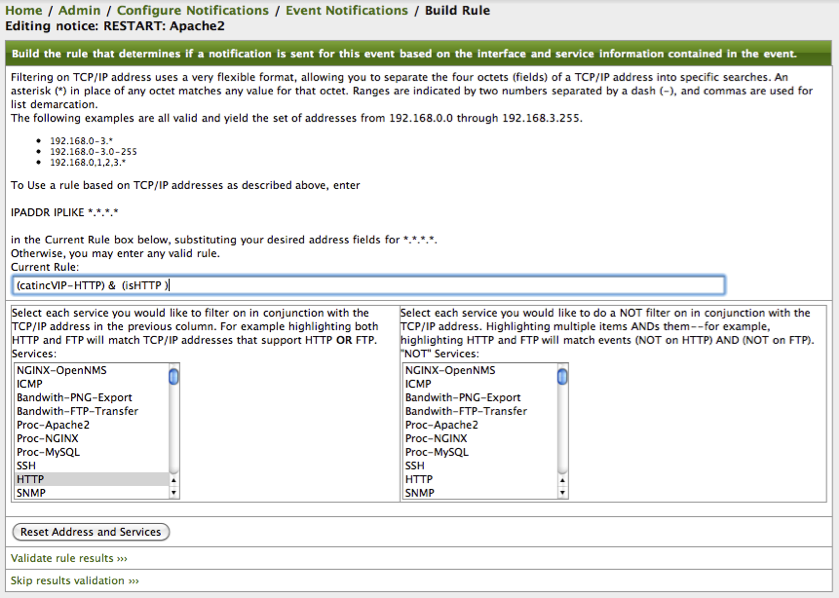
\includegraphics[width=1.0\textwidth]{images/use-cases/service-recovery/notification-rule}
	\caption{Regel für Benachrichtigung für relevante \emph{VIP-HTTP Server}}
	\label{pic:notification-rule-VIP-HTTP}
\end{figure}

Der \emph{Apache2} soll nur für \emph{Nodes} neu gestartet werden die den Service \emph{HTTP} und in der Gruppe \emph{VIP-HTTP} enthalten sind.

\begin{lstlisting}[numbers=none]
(catincVIP-HTTP) & (isHTTP)
\end{lstlisting}

Die Regel kann über \emph{Validate rule } geprüft und dann bestätigt werden. Im nächsten Schritt wird die eigentliche Konfiguration dargestellt. Das Feld \emph{Text Message} hat hier eine besondere Bedeutung. Es enthält den Parameter dem Skript \emph{ssh-restart.sh} mit übergeben wird.

Schlägt das neu starten des \emph{Apache2-Service} fehl, wird eine \emph{SMS} versendet. Diese Benachrichtigung verwendet das \emph{Short Message} Textfeld als Nachrichtentext.

\begin{figure}[H]
	\centering
	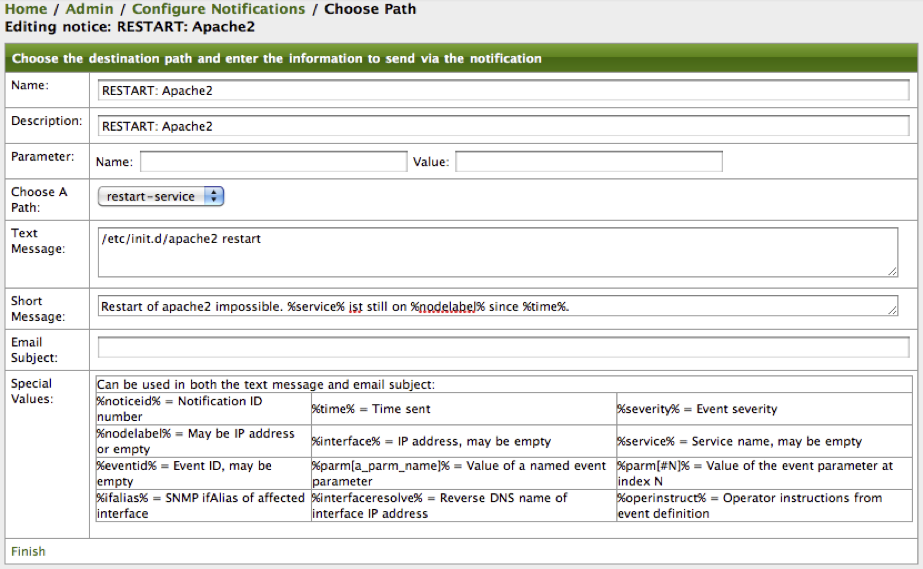
\includegraphics[width=1.0\textwidth]{images/use-cases/service-recovery/notification-text}
	\caption{Text für die Benachrichtigung und \emph{restart service} Kommando.}
	\label{pic:notification-text}
\end{figure}

Es wird das Kommando \emph{/etc/init.d/apache2 restart} an das \emph{notification command} übergeben. Mit dem angelegten \emph{Destination path} können beliebige Dienste neu gestartet werden. Die Meldung in \emph{Short Message} wird nach dem dritten Versuch des Neustarts als \emph{SMS-Text} versendet.
